\documentclass[titlepage, 12pt]{scrartcl}

\usepackage[utf8]{inputenc}

\usepackage{amsmath,amssymb,amsthm}
\usepackage{thmtools}

\usepackage[croatian]{babel}
\usepackage{csquotes}

\usepackage[unicode]{hyperref}
\usepackage{enumitem}
\usepackage{minted}
\usepackage{graphicx}


\MakeOuterQuote{"}


\title{Modeliranje grafovske baze podataka za društvenu mrežu - \emph{Neo4j}}
\author{Karlo Basioli \and 
        Antonela Bogdanić \and 
        Ivan Krcivoj }
\date{Lipanj 2021}

\begin{document}

\maketitle

\tableofcontents

\newpage

\section{Uvod}
Tema ovog projekta je modeliranje grafovske baze podataka za društvenu mrežu koristeći \emph{Neo4j}. Zadatak podrazumijeva odabir programskog jezika za izgradnju grafičkog sučelja, osmišljavanje i implementaciju struktura podataka potrebnih za pisanje kompleksnih upita te generiranje podataka i punjenje same baze. \\
Projekt je u potpunosti izveden koristeći \emph{Python 3.9} programski jezik uz modul \emph{tkinter} za grafičko sučelje i modul \emph{neo4j} koji omogućava spajanje na bazu. \\
U sklopu projekta potrebno je osmisliti upit za predlaganje osoba sličnih po obrazovanju i znanju te upit za predlaganje osoba po samostalno osmišljenom kriteriju.

\newpage
\section{Struktura podataka}
Prvi problem projekta je razrada struktura podataka kojima će društvena mreža biti modelirana. Kao inspiracija gledane su društvene mreže kao što su \emph{Facebook}, \emph{Twitter}, \emph{Instagram}, \emph{LinkedIn} \dots \\
Ove popularne društvene mreže danas broje stotine milijuna korisnika. Unatoč brojnim razlikama u suštini imaju sličnu poantu. Njihov zadaća je povezati korisnike. Ljudi koji koriste ove mreže mogu se međusobno dodavati za prijatelje, pratiti razne grupe, razmjenjivati poruke, dijeliti fotografije i slično. \\
Aspekt koji je gotovo uvijek zajednički je upravo spajanje korisnika. To će biti fokus ovog projekta. Potrebno je osmisliti kako reprezentirati korisnika i njegove veze sa ostalim korisnicima. Također korisnici će biti podijeljeni na smisleni način po edukaciji i njihovim vještinama.

\subsection{Vrhovi}
\subsubsection{Person}
Korisnik će u bazi podataka biti reprezentiran vrhom \emph{Person} sa sljedećim svojstvima:
\begin{itemize}
\begin{samepage}
    \item \textbf{id} identifikacija korisnika
    \item \textbf{name} ime korisnika
    \item \textbf{surname} prezime korisnika
    \item \textbf{gender} spol korisnika
    \item \textbf{date\_of\_birth} datum rođenja korisnika
    \item \textbf{skills} vještine koje korisnik dobija samostalno ili učenjem na fakultetu
    \item \textbf{hobbies} hobiji korisnika
\end{samepage}
\end{itemize}
Svaki \emph{id} postavljen je prilikom generiranja koda te je postavljen kao jedistven u bazi naredbom:
%TODO vidi kako ovo popraviti
\begin{minted}[tabsize=1,breaklines]{cypher}
CREATE CONSTRAINT personIdConstraint ON (person:Person) ASSERT person.id IS UNIQUE;
\end{minted}
Također, kombinacija (\emph{name}, \emph{surname}) je jedinstvena zbog jednostavnosti.
\\ \\
\subsubsection{College}
Kako je važno znati edukaciju korisnika u bazi podataka nalaziti će se i vrh \emph{College} koji predstavlja fakultet te ima sljedeća svojstva:
\begin{itemize}
\begin{samepage}
    \item \textbf{id} identifikacija korisnika
    \item \textbf{name} puno ime fakulteta
    \item \textbf{short\_name} skraćeno ime fakulteta
    \item \textbf{area} područje u koje spada fakultet
    \item \textbf{skills} vještine koje polaznik ovog fakulteta može steći
\end{samepage}
\end{itemize}
Slično kao kod vrha \emph{Person} svojstvo \textbf{id} je jedinstveno. \\
Važna pretpostavka ove baze je da je svaki njen korisnik pohađao fakultet. 
\subsection{Relacije}
\subsubsection{IS\_FRIEND}
Očito važna relacija u ovoj bazi podataka je relacija \emph{IS\_FRIEND}. Ova relacija uspostavlja se između dva vrha sa oznakom \emph{Person} i govori da su ta dva korisnika prijatelji u ovoj društvenoj mreži. \\
Jedini atribut je:
\begin{itemize}
\begin{samepage}
    \item \textbf{start\_date} početak prijateljstva
\end{samepage}
\end{itemize}
Veza nije usmjerena te između dva korisnika postoji najviše jedna veza. \\ \\
\begin{center}
    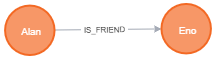
\includegraphics{slike/IS_FRIEND.png}
\end{center}

\subsubsection{SAME\_AREA}
Relacija \emph{SAME\_AREA} povezuje dva fakulteta koja spadaju u isto znanstveno područje. Ova relacija služi za skraćivanje nekih upita te dodatne atribute. \\
Veza također nije usmjerena te dva fakulteta mogu biti povezana najviše jednom ovakvom vezom. \\
U konkretnoj bazi postoje samo tri područja.
\\ \\
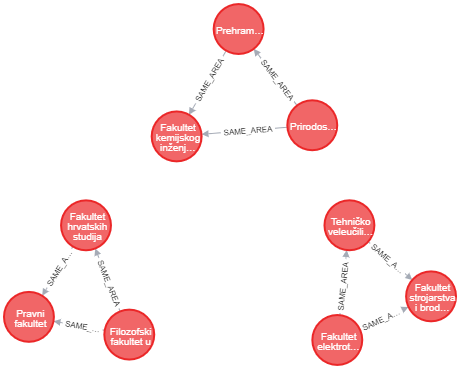
\includegraphics{slike/SAME_AREA.png}

\subsubsection{ATTENDED}
Na kraju postoji i relacija \emph{ATTENDED}. Ovo je prva i jedina jednosmjerna relacija u bazi. Predstavlja vezu između korisnika i fakulteta. Ukoliko se ova dva vrha povezana bridom \emph{ATTENDED} to značni da korisnik pohađa ovaj fakultet. \\
Svojstva ove veze su:
\begin{itemize}
\begin{samepage}
    \item \textbf{enrollment\_year} godina upisa fakulteta
    \item \textbf{graduate\_year} godina završetka fakulteta
    \item \textbf{grade} prosjek ocjena dosadašnjeg studija
\end{samepage}
\end{itemize}
\begin{center}
    
\includegraphics{slike/ATTENDED.png}    
\end{center}

\newpage

\section{Generiranje podataka}
\subsection{Izvori podataka}
\subsection{Kako su podaci generirani}
\newpage

\section{Implementacija aplikacije i grafičko sučelje}
Kao što je već spomenuto za izgradnju aplikacije korišten je programski jezik \emph{Python} zbog velikog broja modula koje posjeduje i jednostavnosti korištenja tih modula. \\
Za interakciju sa bazom korišten je modul \emph{neo4j} dok se grafičko sučelje izgradilo sa modulom \emph{tkinter}.
\subsection{Modul neo4j}
Ovaj modul među nekoliko postojećih \emph{Python} modula za \emph{Neo4j} zato što je i službeno podržavan od strane \emph{Neo4j} baze podataka. \\
Za projekt je napravljena klasa \emph{Database} kao \emph{singleton} kako se ne bi nepotrebno stvarao preveliki broj različitih \emph{drivera}.
\begin{minted}[tabsize=1,breaklines]{python}
class Database:
    __instance = None

    @staticmethod
    def get_instance(path = "database.cfg"):
        if Database.__instance == None:
            Database(path)
        return Database.__instance

    def __init__(self, path):
        if Database.__instance != None:
            raise Neo4jError("This class is a singleton!")
        else:
            #čitanje potrebnih podataka iz .cfg datoteke
            self.driver = GraphDatabase.driver(db_url, auth=(username, password))
            Database.__instance = self

    def close(self):
        self.driver.close()
\end{minted}
Prikazane su samo najosnovnije metode ove klase. \\
Instanca ove klase koristi se za slanje upita na bazu podataka. Jednostavan uzorak koji je praćen kroz cijeli projekt izgleda otprilike ovako:
\begin{minted}[tabsize=1, breaklines]{python}
def query_database(cypher_query, args_dict, path_to_cfg):
    db = Database.get_instance(path_to_cfg)
    
    with db.driver.session() as session:
        result = session.run(cypher_query, args_dict)
    #obrada dobijenih rezultata
\end{minted}
Veliki izazov korištenja ovog modula i projekta općenito bilo je osmisliti kako puniti bazu sa generiranim podacima. Kao što je već spomenuto generirani podaci spremani su u \emph{.csv} datoteke. \\
Deklarativni jezik \emph{cypher} podržava naredbu: 
\begin{minted}{cypher}
LOAD CSV
\end{minted}
Ova naredba omogućava jednostavno učitavanje \emph{.csv} datoteka. Kako bi bilo omogućeno što jednostavnije punjenje baze za različite korisnike ove datoteke se pokretanjem \emph{Python} skripte šalju u \emph{import} direktorij čiji je \emph{path} potrebno zapisati u \emph{database.cfg} datoteku. \\
Upiti za učitavanje vrhova iz baze grade se na sljedeći način:
\begin{minted}[tabsize=1,breaklines]{python}
def get_load_command_entity(self, file_name, header, entity):
    header = header.split(",")
    cypher = f"LOAD CSV WITH HEADERS FROM \"file:///{file_name}\" AS csv_line CREATE (p:{entity}" + "{"
    first = True

    for header_element in header:
        if first:
            cypher += add_attribute(header_element)
            first = False
        else:
            cypher += ", " + add_attribute(header_element)

    cypher += "});"

    return cypher
\end{minted}
Na ovaj način osigurano je jednostavno punjenje baze podataka za svakog korisnika pokretanjem skripti za generiranje podataka, a potom i skripte za punjenje baze.
\subsection{Tkinter}
\newpage

\section{Preporuke}
\subsection{Poslovne preporuke}
\subsection{Osobne preporuke}

\newpage
\section{Zaključak}

\end{document}
